\section[Desenvolvimento]{Desenvolvimento}
\label{cap:desenvolvimento}

Após o planejamento do projeto, foi feito o desenvolvimento de cada etapa.
Para isso, foi feito o desenvolvimento da placa de controle para poder acionar os motores.
Depois disso, o \textit{software} para ler os dados das manetes e enviar os comandos para a placa de controle foi desenvolvido.

A seguir, essas etapas serão detalhadas.

\subsection[Desenvolvimento da placa de controle]{Desenvolvimento da placa de controle}

Primeiramente, foi feito o desenvolvimento da placa de controle dos manipuladores, pois ela será necessária para enviar sinais de movimento para as juntas.
A placa utiliza módulos L293D, Circuitos Integrados (CI) de ponte H, para controlar os motores dos manipuladores.
Cada módulo é capaz de controlar dois motores, portanto foi necessário utilizar 3 CI para todas as juntas.

Para simplificar o controle e evitar problemas de acionamento duplo das entradas das pontes H, foi utilizado o CI 74LS02 como um inversor lógico.
Dessa forma, a placa de controle possui para cada junta uma entrada de \textit{Enable} para ligar/desligar o acionamento da junta, e uma porta de \textit{Direction} para definir a direção de movimentação dela.

Depois de desenvolvida a placa com o auxílio do software \textit{Altium Designer}, ela foi produzida manualmente com o auxílio de tintas fotossensíveis para marcação de trilhas.
Em seguida, foi feita a corrosão das trilhas, a perfuração dos furos e por fim a soldagem dos componentes.
A Figura \ref{fig:placaControle} mostra a placa de controle produzida, com os CI L293D e 74LS02, e a Figura \ref{fig:placaControleEsquematico} mostra o esquemático da placa.

\begin{figure}[H]
    \begin{minipage}{.5\textwidth}
        \centering
        \caption{Placa de controle produzida}
        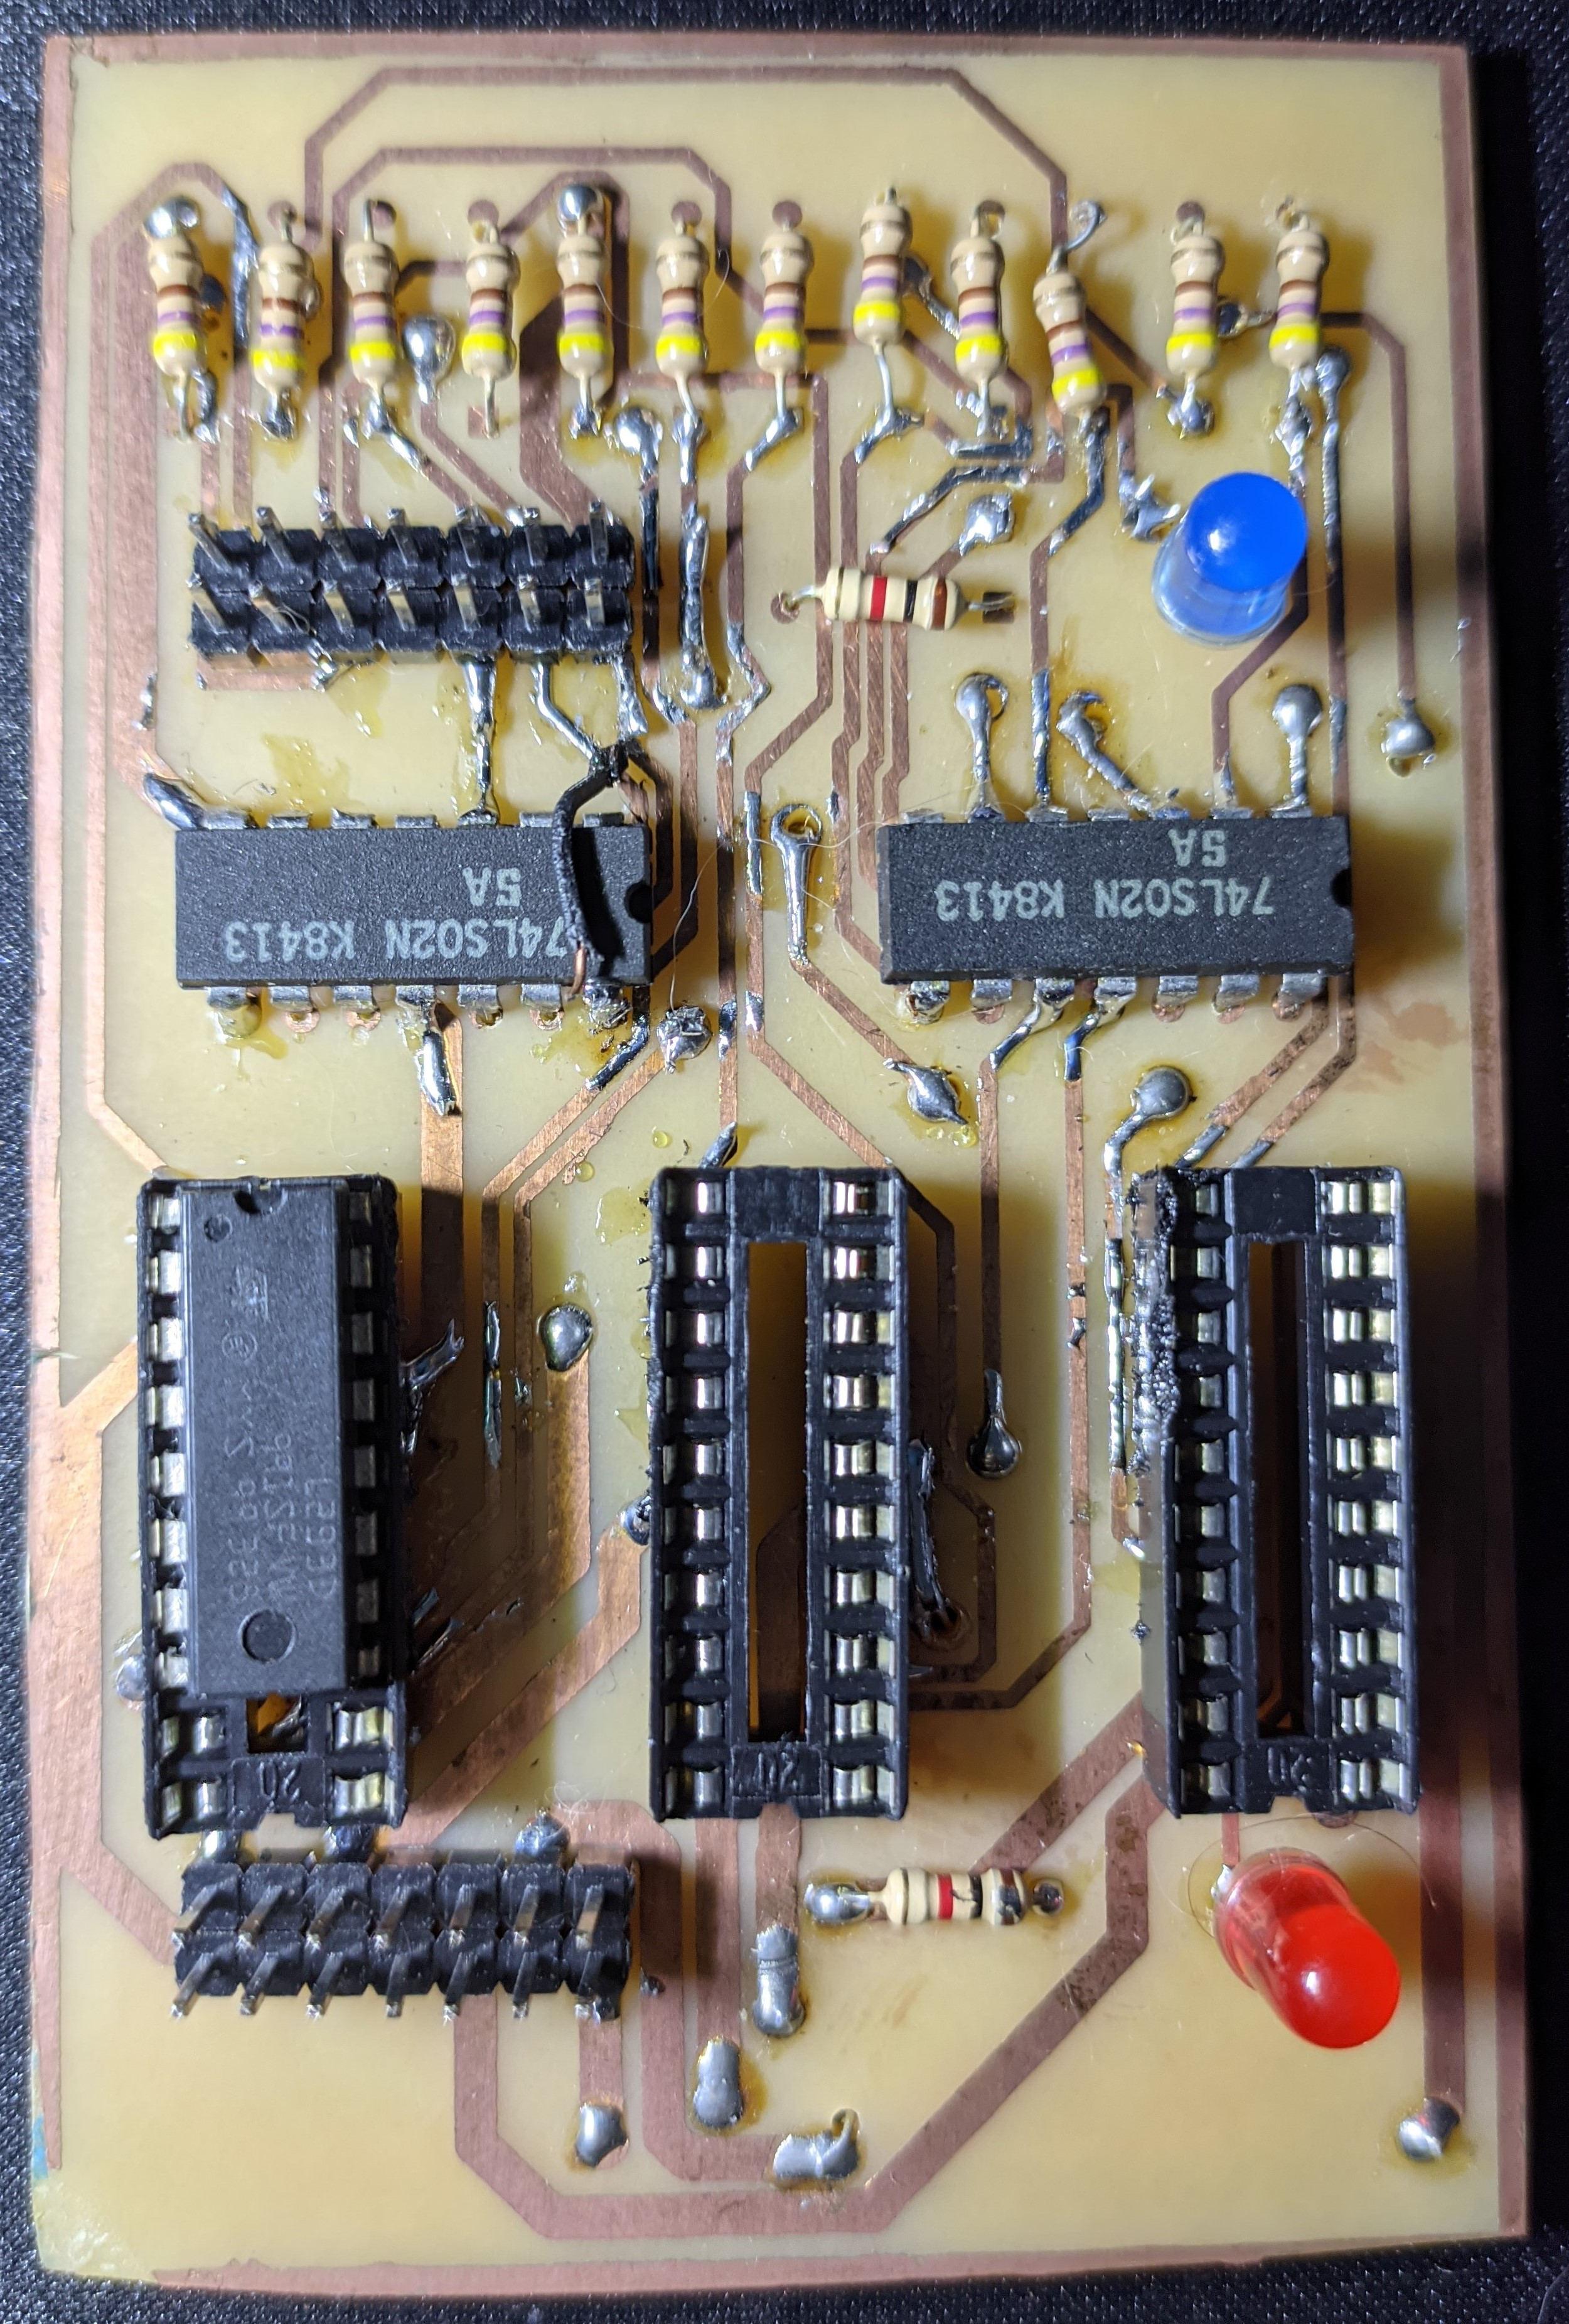
\includegraphics[keepaspectratio=true, width=0.9\linewidth]
            {img/placa-controle.jpg}
        \fonte{Do próprio autor}
        \label{fig:placaControle}
    \end{minipage}%
    \begin{minipage}{.5\textwidth}
        \centering
        \caption{Esquemático da placa de controle}
        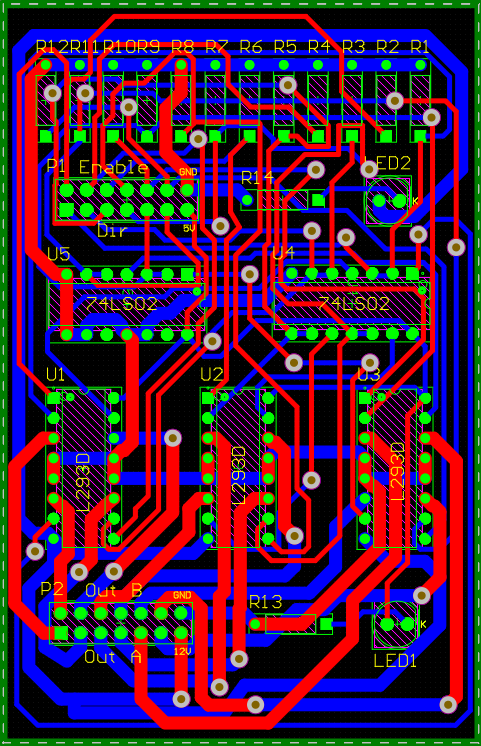
\includegraphics[keepaspectratio=true, width=0.9\linewidth]
            {img/placa-controle-esquematico.png}
        \fonte{Do próprio autor}
        \label{fig:placaControleEsquematico}
    \end{minipage}%
\end{figure}

\subsection[Leitura das manetes]{Leitura das manetes}

Em seguida, foi desenvolvido um \textit{software} com o microcontrolador para realizar a leitura dos dados das manetes.
Cada manete possui dois \textit{joysticks} de dois eixos e um botão.
Para realizar a leitura dos eixos dos \textit{joysticks}, foram utilizadas as entradas analógicas do microcontrolador.
Para realizar a leitura do botão, foi utilizada uma entrada digital.

Os eixos dos \textit{joysticks} são utilizados para mover o manipulador, por isso os valores lidos são utilizados para alterar a posição desejada de cada junta.
Para aprimorar a usabilidade deles, foi implementada uma \textit{deadzone}, que é uma área em que o valor lido é considerado como zero, para evitar que o manipulador se movimente sem a intenção do usuário.

\subsection[Controle dos motores]{Controle dos motores}

Para controlar os motores, foi utilizado como base o \textit{software} desenvolvido anteriormente para ler os dados das manetes.
Primeiramente foi implementada a leitura da posição atual de cada junta, utilizando as entradas analógicas do microcontrolador.

Depois disso, foi feita a configuração de uma interrupção por \textit{timer} acionada a cada 10ms, para realizar o controle dos motores.
Nessa interrupção, é feita a leitura da posição de cada junta, execução de um PID para o cálculo da largura de pulso e envio desse sinal PWM para a placa de controle.